\documentclass{article}
\usepackage{neurips_2025}
\usepackage[utf8]{inputenc}
\usepackage[T1]{fontenc}
\usepackage{hyperref}
\usepackage{url}
\usepackage{booktabs}
\usepackage{amsmath}
\usepackage{amssymb}
\usepackage{graphicx}
\usepackage{xcolor}

\title{Written Values Are Read Back:\\The Chain of Thought as Addressable Memory}

% Anonymous submission: author block suppressed by the default style option.
\author{%
  Anonymous Author(s)\\
  Affiliation\\
  \texttt{email}\\
}

\begin{document}

\maketitle

\begin{abstract}
When a language model writes an intermediate value during multi-step reasoning, the written token could carry the computation forward or describe work done elsewhere in the network. Prior work has shown, on a fine-tuned model and on multiplication and dynamic-programming tasks, that intervening on such tokens changes the answer. We test the question on unmodified pretrained models across four families and two task formats, and localize the mechanism. Overwriting the internal state at a written value's token with the state a different number would have produced, while leaving the visible text unchanged, makes the final answer track the never-written value in 74 to 100 percent of cases (six models, arithmetic and narrative tasks), while a size-matched random perturbation moves the answer in under 3 percent. Blocking attention from later positions to that one token drops the answer's dependence on it to near zero on four models in three families, while blocking a neighboring token, a random prompt token, or an earlier written value leaves it unchanged; the model continues to produce fluent, parseable answers, so the intervention removes access to the value rather than disabling generation. Two values planted at two positions compose into their sum, which appears nowhere in the input. Models consult this stored value by default, and which prompt evidence leads them to recompute it instead differs by model. On serially dependent state that a model cannot cheaply regenerate, the written trace is the memory the computation reads, which bears directly on whether reading a model's chain of thought reveals what it computed.
\end{abstract}

\section{Introduction}

Oversight of language-model reasoning often assumes that the text a model writes reflects the computation it performs. Faithfulness studies have shown that stated reasoning and internal computation can diverge~\citep{turpin2023unfaithful, lanham2023faithfulness}. This leaves a specific mechanistic question open: when a model writes ``after step 5 the value is 452'' and later uses 452, does the written token cause the later use, or does the computation happen elsewhere and the token record it?

Causal interventions on written reasoning tokens are not new. \citet{shih2026registers} patch internal representations of scratchpad state on a fine-tuned model and report downstream following of 0.80 to 0.91, and \citet{zhu2025variables} intervene on value-storing tokens in multiplication and dynamic-programming tasks. We extend this in four directions. First, the effect holds on \emph{unmodified} pretrained models across four families (Qwen, Phi, OLMo, DeepSeek-R1-Distill) and two task formats. Second, we localize the read to attention directed at the value's own token, with matched-token controls and a fluency check that rules out simply disabling generation. Third, planted values compose: two positions act as independent stores. Fourth, we map when a model recomputes a value instead of reading it, and find the answer is model-specific rather than a single scale trend.

The central result is that a written intermediate value is held at its token position as state that later computation reads back through attention, and that this stored value, not the visible text and not the value the problem implies, determines the answer. We establish it with three interventions on one protocol (Figure~\ref{fig:protocol}): edit the visible text, overwrite the internal state, and block the attention that reads the token.

\begin{figure}[t]
\centering
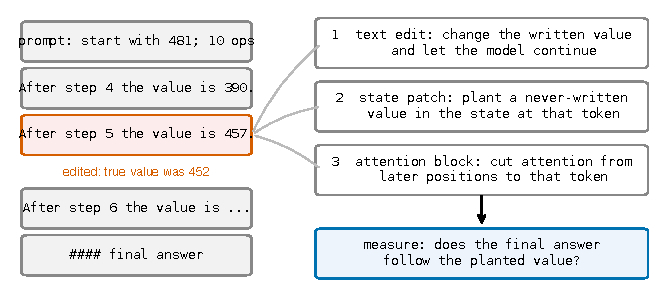
\includegraphics[width=0.95\linewidth]{figures/f1_protocol.pdf}
\caption{The edit-and-continue protocol. A correct worked solution is truncated after one edited value line, and the model continues. Three interventions act on the edited value: changing the visible token, overwriting the internal state at that token with the state a different value would produce, and blocking attention from later positions to that token. In each case we measure whether the final answer follows the planted value.}
\label{fig:protocol}
\end{figure}

\section{Setup}

\paragraph{Tasks.} We use two families of problems for which every intermediate value is known by construction, so the effect of any edit is computable exactly. Arithmetic chains start from a three-digit number and apply $d$ signed two-digit additions and subtractions. Narrative state-tracking problems describe a character whose count of some item changes through varied events, with varied names, items, verbs, and sentence forms. In both, the model writes one line per step giving the running value.

\paragraph{Protocol.} We take a correct worked solution, change the value at one step $j$ by a small amount, truncate immediately after the edited line, and let the model continue. A no-edit truncation measures the sampling noise floor, which is 0.00 throughout. Answers are parsed from a fixed final-line format, and unparseable outputs are counted separately.

\paragraph{Interventions.} The \emph{text edit} changes only the visible token. The \emph{state patch} leaves the text intact and overwrites the residual stream at the value's token position, across a band of middle layers, with activations captured from a run in which a different value was written there. The \emph{attention block} adds a mask so that no position after the edit can attend to the value's token.

\paragraph{Models and reporting.} White-box experiments run on Qwen3-4B, Qwen2.5-7B-Instruct, Phi-3-medium, OLMo-2-7B-Instruct, and DeepSeek-R1-Distill-Qwen 7B and 14B. Frontier models (DeepSeek V3.2, Claude Sonnet 4.5, Llama 3.3 70B) are tested behaviorally through assistant prefill. Generation uses temperature 0.6 and top-$p$ 0.95, with five samples per item where sampling is used; the noise floor is measured under the same settings. Reported intervals are 95 percent bootstrap intervals resampling over items. We report intervals rather than significance tests and apply no multiple-comparison correction; the effects that carry the argument are separated from their controls by margins far larger than the intervals. Sample sizes are 46 to 600 per condition. Model revisions, prompts, exact layer bands, and per-run configurations are in the appendix, and code and data will be released.

\section{The state at a written token holds the value}
\label{sec:patch}

Editing the visible text alone changes the final answer on most items. The state patch decomposes this effect (Table~\ref{tab:patch}). Restoring the correct internal state while the visible text still shows a corrupted value returns the answer to correct in 0.88 to 1.00 of cases. Planting a third value that appears nowhere in the text makes the answer track that value in 0.70 to 1.00 of cases. The size-matched random control is at or below 0.01 for the instruction-tuned models. The effect persists with chain length: on Qwen3-4B the planted value is followed at 0.98, 0.97, and 0.95 for chains of 5, 20, and 40 steps.

\begin{table}[t]
\centering
\small
\caption{State patch on arithmetic chains at ten steps. Rates are conditioned on items where the text edit was followed (that rate is the first column), so cross-model comparison of the later columns should account for it. Brackets are 95 percent bootstrap intervals. The two reasoning-distilled models re-solve the problem after their reasoning phase, which raises their random-control reversion; that re-derivation can only produce the correct answer and so does not affect the planted-value column.}
\label{tab:patch}
\begin{tabular}{lccccc}
\toprule
model & text edit followed & restore correct & plant new value & random control & $n$ \\
\midrule
Qwen3-4B & 0.98 [0.95, 1.00] & 1.00 [1.00, 1.00] & 1.00 [0.99, 1.00] & 0.00 [0.00, 0.00] & 106 \\
Qwen2.5-7B-Instruct & 0.85 [0.80, 0.90] & 0.97 [0.92, 1.00] & 0.74 [0.67, 0.81] & 0.00 [0.00, 0.01] & 93 \\
Phi-3-medium & 0.94 [0.90, 0.98] & 0.98 [0.95, 1.00] & 0.94 [0.91, 0.97] & 0.00 [0.00, 0.00] & 102 \\
OLMo-2-7B & 0.85 [0.79, 0.91] & 0.88 [0.82, 0.94] & 0.93 [0.88, 0.97] & 0.00 [0.00, 0.00] & 100 \\
R1-distill-7B & 0.60 [0.53, 0.66] & 1.00 [0.99, 1.00] & 0.76 [0.68, 0.84] & 0.30 [0.22, 0.39] & 65 \\
R1-distill-14B & 0.44 [0.36, 0.52] & 0.99 [0.98, 1.00] & 0.70 [0.61, 0.80] & 0.21 [0.13, 0.29] & 46 \\
\bottomrule
\end{tabular}
\end{table}

\paragraph{The reasoning-distilled models.} R1-distill-7B and 14B show an elevated random-control reversion (0.30 and 0.21) because they re-solve the problem after their reasoning phase. In a logged sample of the reverting cases, the continuation re-derives from the problem's starting value rather than correcting the value in place. Re-solving can only produce the correct answer, so it inflates the random control without touching the planted-value column, where the answer is a value the model never wrote and the problem never implies. R1-distill-1.5B is excluded: at 12 usable items its competence is too low to interpret.

\paragraph{Not the arithmetic template.} On the narrative task the pattern replicates. Planting a never-written count is followed at 0.83 [0.75, 0.90] on Qwen3-4B and 0.86 [0.79, 0.92] on Phi-3-medium, restoring the correct state returns the answer at 0.89 and 0.94, and the random control is 0.00 in both ($n=86$ and 89 conditioned items). The stored value is a property of written state, not of one surface form.

\paragraph{Two positions act as independent stores.} In a task with two counters summed at the end, we plant a never-written value at each of the two final positions. Each single-position patch yields the corresponding mixed sum (0.94 and 0.93 on Qwen2.5-7B, 0.89 and 0.93 on Qwen3-4B). Planting both yields their joint sum at 0.90 and 0.88, at or above the product of the single-position rates (0.89 and 0.83). The size-matched random patch leaves the clean answer in place (0.96 and 0.95), and answers matching only one of the two planted values occur at 0.01. The model reports a number that exists nowhere in its input, assembled from two independently set stores.

\section{The value is read back through attention to its token}
\label{sec:knockout}

Blocking attention from all positions after the edit to the edited value's token collapses the answer's dependence on that value (Table~\ref{tab:knockout}). The same block applied to the adjacent words on the same line, to a random operand in the prompt, or to an earlier step's written value leaves the dependence at its no-block level. Blocking the operand that the next step needs breaks the arithmetic itself, giving answers that match neither the edit nor the correct value. The collapse holds on four models across three families and on both task formats (Figure~\ref{fig:knockout}).

\begin{figure}[t]
\centering
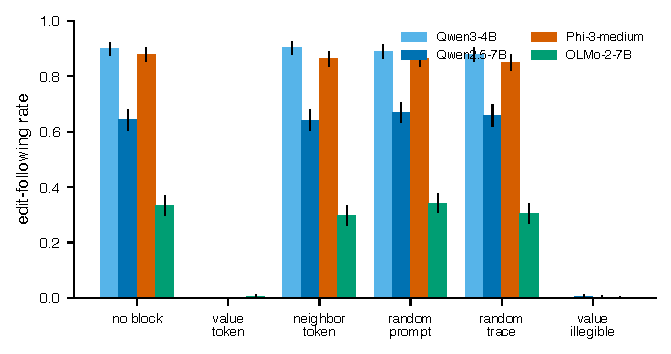
\includegraphics[width=0.75\linewidth]{figures/f3_knockout.pdf}
\caption{Rate at which the answer follows the edited value when attention to a chosen token is blocked. Blocking the value's own token collapses following on every model; blocking a neighboring token, a random prompt token, or an earlier written value leaves it at the no-block level. Error bars are 95 percent bootstrap intervals.}
\label{fig:knockout}
\end{figure}

\begin{table}[t]
\centering
\small
\caption{Attention block on arithmetic chains: rate at which the answer follows the edited value under each blocked target. Value blocks the edited value's token; neighbor, random prompt token, and earlier written value are matched controls. OLMo-2-7B has a low no-block rate in this format but the same contrast. The natural-language task shows the same collapse (Qwen3-4B 0.730 to 0.007; Phi-3-medium 0.720 to 0.003).}
\label{tab:knockout}
\begin{tabular}{lccccc}
\toprule
model & no block & value token & neighbor & random token & earlier value \\
\midrule
Qwen3-4B & 0.900 & 0.000 & 0.903 & 0.778 & --- \\
Qwen2.5-7B-Instruct & 0.643 & 0.000 & 0.640 & 0.670 & 0.658 \\
Phi-3-medium & 0.880 & 0.000 & 0.863 & 0.865 & 0.850 \\
OLMo-2-7B & 0.333 & 0.005 & 0.297 & 0.342 & 0.305 \\
\bottomrule
\end{tabular}
\end{table}

\paragraph{The block removes the value, not the ability to generate.} Under the value-token block the unparseable-output rate stays at 0.000 (0.040 on OLMo-2-7B, equal to its no-block rate). The model produces a fluent, parseable number; that number simply matches neither the edited value nor the correct one, because the model computes forward from a value it can no longer retrieve. The intervention removes access to the specific value rather than disabling generation near that position.

\paragraph{Read-back is the preferred path, not the only one.} Replacing the value's characters with dots, without touching attention, also removes following, but differently: the Qwen models reconstruct the value from the previous line and return the correct answer 60 to 73 percent of the time, while Phi-3-medium does not recover (0.00). When the token is present the model reads it; when it is unreadable, some models can rebuild it and by default do not.

\paragraph{What this does and does not establish.} The block masks the value's token at every layer, and the state patch overwrites a band of middle layers. These interventions show that the value at the written token is causally load-bearing and that attention to that token is the conduit. They do not yet localize the read to a specific layer range. A layer-resolved sweep, patching and masking single layers and thirds of the network, is the natural next step and would separate a compact retrieval circuit from a distributed one; we report it as the primary open item. The controls above rule out the cruder alternatives available without it: the effect is specific to the value token rather than any trace token, and the model remains fluent, so ``following drops to zero'' is not merely broken generation.

\section{When the written value is checked}
\label{sec:verify}

Models follow edited values by default. Whether prompt evidence leads a model to recompute a value instead depends on the model and on the kind of evidence, and we did not find it to be a single trend in model capability.

On DeepSeek V3.2, editing a value the prompt only implies is followed at 0.93, while editing a value the prompt generatively defines (the prompt states the two numbers whose sum becomes the running value) is reverted to the correct answer at 0.43. The check is targeted: with the defining sentence present but the edit two steps away from the defined value, following returns to 0.96, equal to the implied-value case. Claude Sonnet 4.5 checks a wider range of evidence, reverting most when a stated checkpoint is the value's only source. Llama 3.3 70B follows edits at 0.97 whether or not the value is prompt-defined, despite being able to solve the same chains from scratch, so capacity to recompute does not imply checking. Qwen models at 4B and 7B never revert.

These conditions come from separate experiments with different trace lengths and item sets; each within-experiment contrast is controlled, and we do not claim a single ordered scale across them. The behavioral edit-following rates on frontier models (R1-distill-7B 0.42, V3.2 0.78, Sonnet 4.5 0.97 on prompt-underivable chains) do not extend monotonically to Llama 3.3 70B at 0.97, so we do not claim that trace-dependence increases with capability in general. The mechanistic results of Sections~\ref{sec:patch} and~\ref{sec:knockout} are established on the white-box models; the frontier results are behavioral.

\section{Scope}

The mechanism concerns state a model cannot cheaply regenerate from the prompt. The same edit-and-continue test on natural benchmark problems bounds it: on GSM8K worked solutions, editing an intermediate value changes the answer at 0.10 on V3.2 and 0.87 on Qwen3-4B, because a benchmark intermediate is often one operation from numbers still in the prompt, and whether a model rereads it or recomputes it depends on the model's own capacity. Written values act as memory for state that recomputation cannot cheaply reconstruct, and much of benchmark arithmetic does not have that character.

\section{Related work}

Our interventions build on causal tracing and activation patching~\citep{meng2022rome} and causal abstraction~\citep{geiger2021causal}. \citet{heimersheim2024patching} caution that broad patches conflate ``this component matters'' with deleting information at a position, which motivates the layer sweep we identify as the open item. The closest empirical work intervenes on written reasoning tokens: \citet{shih2026registers} on a fine-tuned model and \citet{zhu2025variables} on multiplication and dynamic-programming tasks. We differ in testing unmodified pretrained models across four families and two task formats, localizing the read to attention to the value token with matched controls and a fluency check, showing composition, and mapping when the record is checked. Faithfulness studies established that stated reasoning and internal computation can diverge~\citep{turpin2023unfaithful, lanham2023faithfulness}, and filler-token results show computation can proceed through uninformative tokens~\citep{pfau2024dot}; these bound our claim to state a model cannot regenerate internally. Expressivity theory predicts that long dependency chains must live in the generated text~\citep{merrill2024expressive}, and Self-Notes~\citep{lanchantin2023selfnotes} studies writing as memory behaviorally.

\section{Limitations}

The state patch overwrites a band of middle layers and the attention block masks all layers, so the read is not yet localized to a specific depth; this is the primary revision item. The white-box causal evidence is at 4B to 14B scale, and the frontier evidence is behavioral. Tasks are arithmetic and narrative-count chains with exact ground truth; richer state such as code or multi-entity plans is untested. The checking-policy results in Section~\ref{sec:verify} draw on conditions from separate experiments and support within-experiment contrasts rather than a single ordered scale. The state patch is controlled against a size-matched random vector; a structured control that plants a valid activation for a different value would further separate value content from generic activation shape.

\section{Conclusion}

On two task formats and across four model families, a value written in a chain of thought is held at its token position as state that later computation reads back through attention, and that stored value determines the answer even when it appears nowhere in the text and contradicts what the problem implies. Two positions act as independent stores. Models read this state by default, and what leads them to recompute instead is model-specific. For oversight, the consequence is scoped and concrete: on serially dependent state a model cannot cheaply regenerate, the written trace is the memory the computation uses, so reading the trace observes the computation; on state the model can regenerate, the trace and the computation can diverge.

\bibliographystyle{plainnat}
\bibliography{references}

\end{document}
